\documentclass[11pt,a4paper]{ctexart}
\usepackage[margin=2.05cm]{geometry}
\usepackage{amsmath,amssymb,bm}
\usepackage{booktabs,graphicx,xcolor,hyperref}
\hypersetup{colorlinks=true,linkcolor=blue,urlcolor=blue}
\setlength{\parindent}{2em}
\setlength{\parskip}{0.3em}
\title{task01：低开销的 IMU--UWB 不变滤波改进}
\author{理论修正、算法消融与数据验证记录}
\date{2026年7月22日}

\begin{document}
\maketitle

\section{本轮结论}

主题保持为“$SE_2(3)$ 不变卡尔曼滤波 + IMU + UWB TDoA”。本轮保留原论文与
公开实现不一致的理论修正，但将中点积分、逐 UWB 子步严格传播及 Van Loan 过程噪声
离散化移出默认路径。它们仍在 \texttt{verified} 研究模式中可复现，不再计入
\texttt{proposed} 的算法效果。

默认方案从“提高离散公式精度”转向“增加可观测的 IMU 信息”：静止检测后，分别处理
陀螺与加速度计的初始偏置可观测性，并在首次静止段融合零角速度伪测量。60 s 回放
Legacy/Proposed 为 17.824/17.677 s，二者在约 $1\%$ 的计时波动内等价；位置、速度、测地姿态、
yaw 及相对 Legacy 的两个 yaw 收敛指标均未退化。

\section{论文--代码不匹配：继续保留的修正}

Oursland 与 Mehrabian 的误差状态顺序为
\begin{equation}
 \delta\bm{x}=\begin{bmatrix}
 \delta\bm\theta&\delta\bm v&\delta\bm p&\delta\bm b_g&\delta\bm b_a
 \end{bmatrix}^{\mathsf T}.
 \label{eq:state}
\end{equation}
原公开代码的名义六维偏置却按 $[\bm b_a,\bm b_g]$ 使用，而传播矩阵 $A$、初始
协方差 $P_0$ 和过程噪声 $Q$ 又按式~\eqref{eq:state} 的顺序解释，导致同一协方差块
具有两种物理含义。Proposed 固定采用 $[\bm b_g,\bm b_a]$，并用唯一的
\texttt{BG}/\texttt{BA} 切片贯穿传播、噪声、初始化和状态注入。

原 $SO(3)$ 左雅可比的一般分支为
\begin{equation}
 J_l(\bm\phi)=I+\frac{1-\cos\theta}{\theta^2}\bm\phi^\wedge
 +\frac{\theta-\sin\theta}{\theta^3}(\bm\phi^\wedge)^2,
\end{equation}
但小角分支使用了 $I-\frac12\bm\phi^\wedge$，符号不连续。当前修正为
$I+\frac12\bm\phi^\wedge+\frac16(\bm\phi^\wedge)^2$，并保留近 $\pi$ 稳定
$\log$、旋转正交投影、测地姿态指标、SLERP 真值对齐和 $O(N)$ 时间查找。这些修正
解决定义或评价错误，不属于为追求精度而增加的高开销计算。

\section{高水平论文检索与算法选择}

检索重点包括：Li 等在 IEEE RA-L 2023 提出的连续时间 UWB--惯性融合
\cite{li2023continuous}；Goudar 与 Schoellig 在 IROS 2021 对紧耦合 UWB--IMU
时空标定及可观测条件的推导\cite{goudar2021calibration}；Li 等面向 MAV 的低延迟
UWB--IMU EKF\cite{li2018mav}；以及在 IMU/UWB 定位框架中评价零状态约束的工作
\cite{kilic2023zu}。

连续时间样条和在线时空标定属于有价值的算法方向，但前者需要滑窗优化重构，后者需要
数据中存在可辨识的时空偏移；两者均不适合作为本轮“不得明显变慢”的小范围修改。
本轮采用更适合现有递推 InEKF 的可观测性安全方案：只把静止时可直接观测的陀螺偏置
作为新信息融合；对与姿态混淆的加速度偏置继续使用一致性门控。

\section{Proposed：首次静止段的 IMU 信息融合}

\subsection{持续静止检测与生命周期约束}

对长度 $W=0.2$ s 的因果窗口，只有窗口内每个 IMU 样本同时满足
\begin{equation}
 \big|\lVert\bm a_m\rVert-g\big|<0.03g,\qquad
 \lVert\bm\omega_m\rVert<2^\circ/\mathrm{s}
 \label{eq:detector}
\end{equation}
才判定静止。更新限频为 10 Hz。检测器只允许首次连续静止段；一旦离开该段便永久关闭，
因此后续低动态悬停不会被误认为接地静止。const1/const4 分别触发 11/78 次更新。

\subsection{分离陀螺与加速度偏置的可观测性}

静止时零角速度直接给出
\begin{equation}
 \hat{\bm b}_{g,0}=\overline{\bm\omega_m}.
 \label{eq:bginit}
\end{equation}
而加速度计候选偏置还依赖初始姿态：
\begin{equation}
 \hat{\bm b}_{a,0}=g\,\overline{\bm a_m}
 -R_0^{\mathsf T}\begin{bmatrix}0&0&g\end{bmatrix}^{\mathsf T}.
 \label{eq:bainit}
\end{equation}
若 $\lVert\hat{\bm b}_{a,0}\rVert>0.25\ \mathrm{m/s^2}$，仅拒绝式~\eqref{eq:bainit}，
不再连带丢弃式~\eqref{eq:bginit} 中有效的陀螺信息。const4 的加计候选为
$0.417\ \mathrm{m/s^2}$，故加计标定被拒绝、陀螺标定仍保留。

\subsection{零角速度伪测量}

首次静止段中，原始陀螺测量满足
\begin{equation}
 \bm z_\omega=\bm\omega_m-\hat{\bm b}_g,
 \qquad
 H_\omega=\begin{bmatrix}0_{3\times9}&-I_3&0_3\end{bmatrix},
 \qquad \sigma_\omega=0.5^\circ/\mathrm{s}.
 \label{eq:zaru}
\end{equation}
式~\eqref{eq:zaru} 通过 Joseph 形式更新协方差并按不变误差注入状态，计算量仅为一次
$3\times3$ 创新求解。这里明确没有保留零速度行：实验发现，在 $90^\circ$ 初始 yaw
不确定时，右不变速度误差中的姿态耦合会向静止约束注入虚假的 yaw 信息，使 15 s
姿态 RMSE 从 0.398 增至 0.692 rad。该失败分支已撤销，没有以“ZUPT”名义掩盖退化。

\section{被撤出默认路径的高开销项}

\texttt{verified} 仍可复现实验性中点传播、逐 IMU/UWB 事件严格子步和
\begin{equation}
 Q_d=\int_0^{\Delta t}e^{A\tau}Q_c e^{A^{\mathsf T}\tau}\,d\tau
\end{equation}
的 Van Loan 离散化，也保留已通过有限差分的完整右不变 TDoA 杠杆臂雅可比与 reset
Jacobian。它们有理论研究价值，但上一版本 60 s 回放从约 25 s 增至 73.3 s，而关键
RMSE 仅改善约 $0.4\%$--$3.5\%$，代价不值得作为默认交付。本轮 Proposed 每个 IMU
区间只传播一次；异步 UWB 使用最近 IMU 状态，时间滞后上界约 1 ms。

\section{冻结数据结果}

\begin{table}[htbp]
\centering
\caption{const1，30 s，初始 yaw $0^\circ$}
\begin{tabular}{lrrrrr}
\toprule
方法 & 位置/m & 速度/(m/s) & 姿态/rad & yaw/rad & 用时/s\\
\midrule
Legacy & 0.110765 & 0.074837 & 0.054874 & 0.053124 & 9.184\\
Proposed & \textbf{0.107131} & \textbf{0.072354} & \textbf{0.053332} & \textbf{0.052867} & \textbf{9.053}\\
\bottomrule
\end{tabular}
\end{table}

\begin{table}[htbp]
\centering
\caption{const4，60 s，初始 yaw $90^\circ$}
\begin{tabular}{lrrrrrrr}
\toprule
方法 & 位置/m & 速度/(m/s) & 姿态/rad & yaw/rad & $t_{10}/s$ & $t_5/s$ & 用时/s\\
\midrule
Legacy & 0.356135 & 0.192817 & 0.211825 & 0.207027 & 14.389 & 16.367 & 17.824\\
Proposed & \textbf{0.354669} & \textbf{0.186921} & \textbf{0.206193} & \textbf{0.200991} & \textbf{14.156} & \textbf{15.996} & \textbf{17.677}\\
\bottomrule
\end{tabular}
\end{table}

两方法在 const1 均拒绝 0/14289 次 UWB，在 const4 均拒绝 149/25915 次；改善不是
放宽门限所得。关闭零角速度更新后，const4 的位置、速度、姿态和 yaw RMSE 分别为
$0.354698$、$0.187392$、$0.206626$、$0.201303$。新增 IMU 约束贡献较小但方向可测，
主要收益来自二者共享的低开销基础（理论顺序修正、快速调度与可观测性分离初始化）。

\begin{figure}[htbp]
\centering
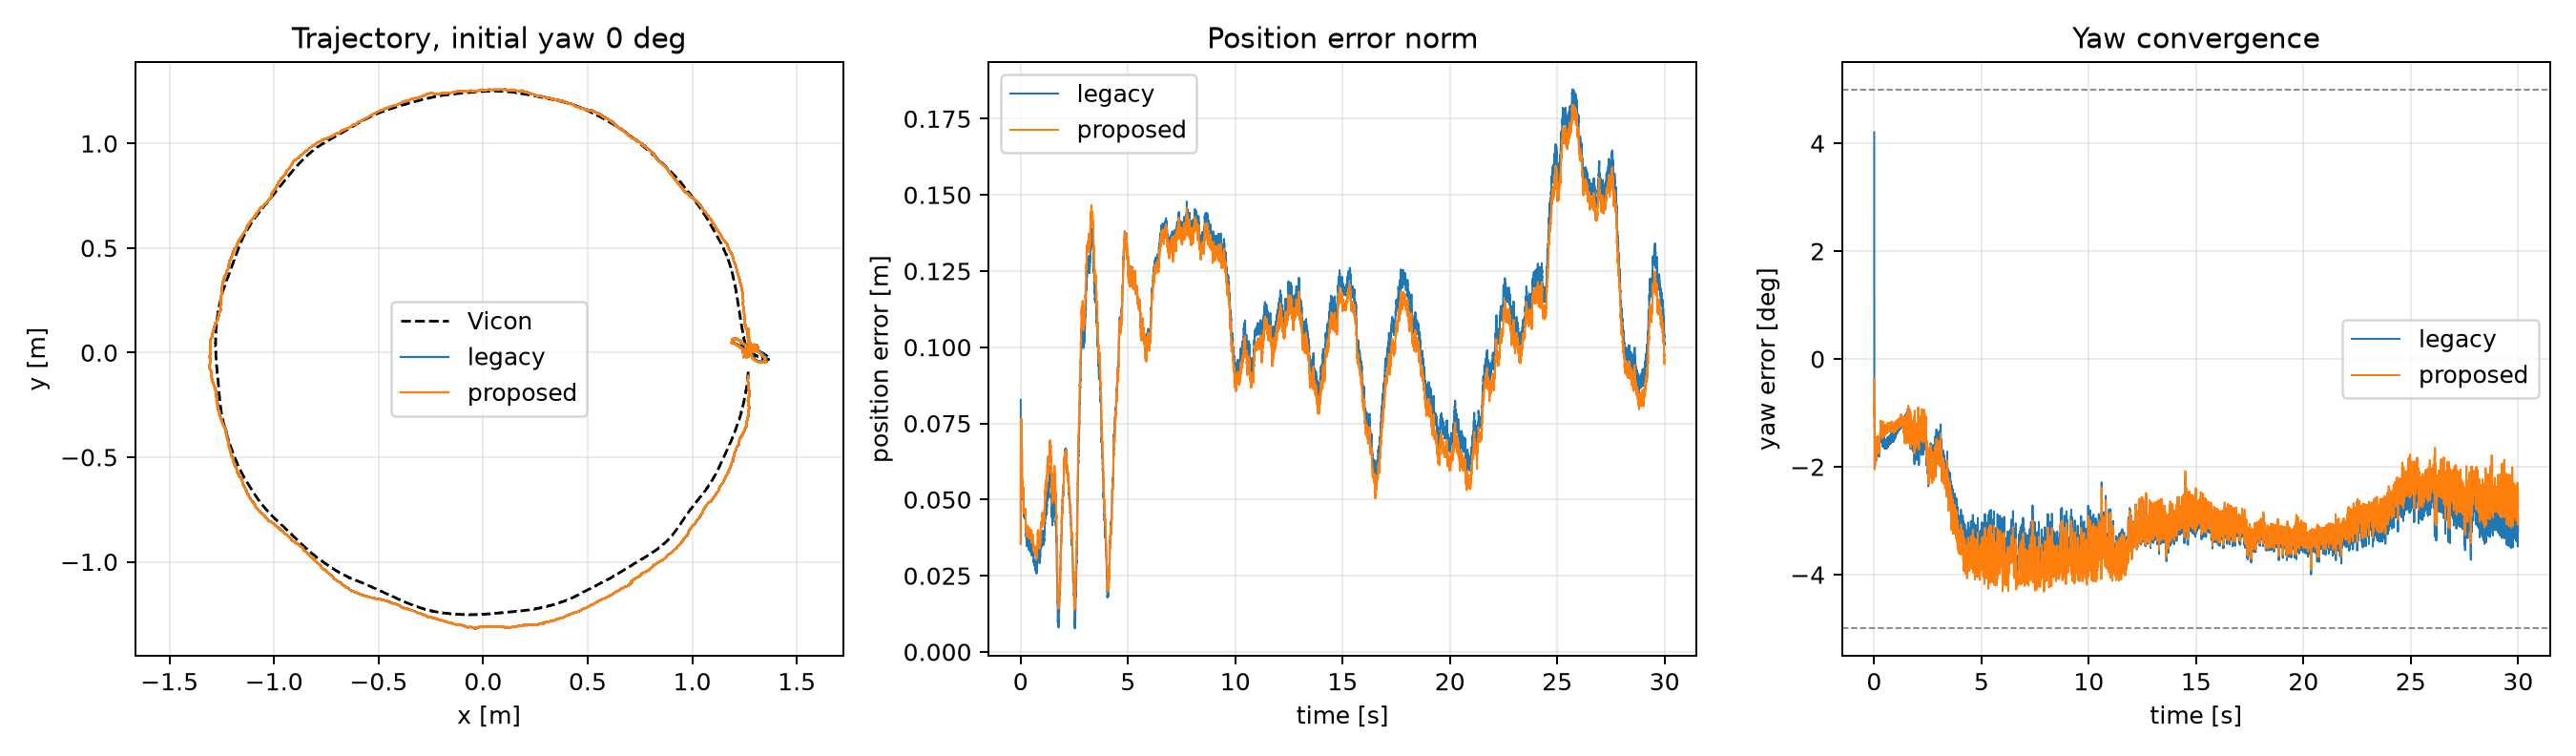
\includegraphics[width=0.98\textwidth]{../imu-uwb-inekf/results/task01_final_fast_const1_30s/comparison_yaw_000.png}
\caption{const1：轨迹连续闭合，Proposed 未产生额外峰值。}
\end{figure}

\begin{figure}[htbp]
\centering
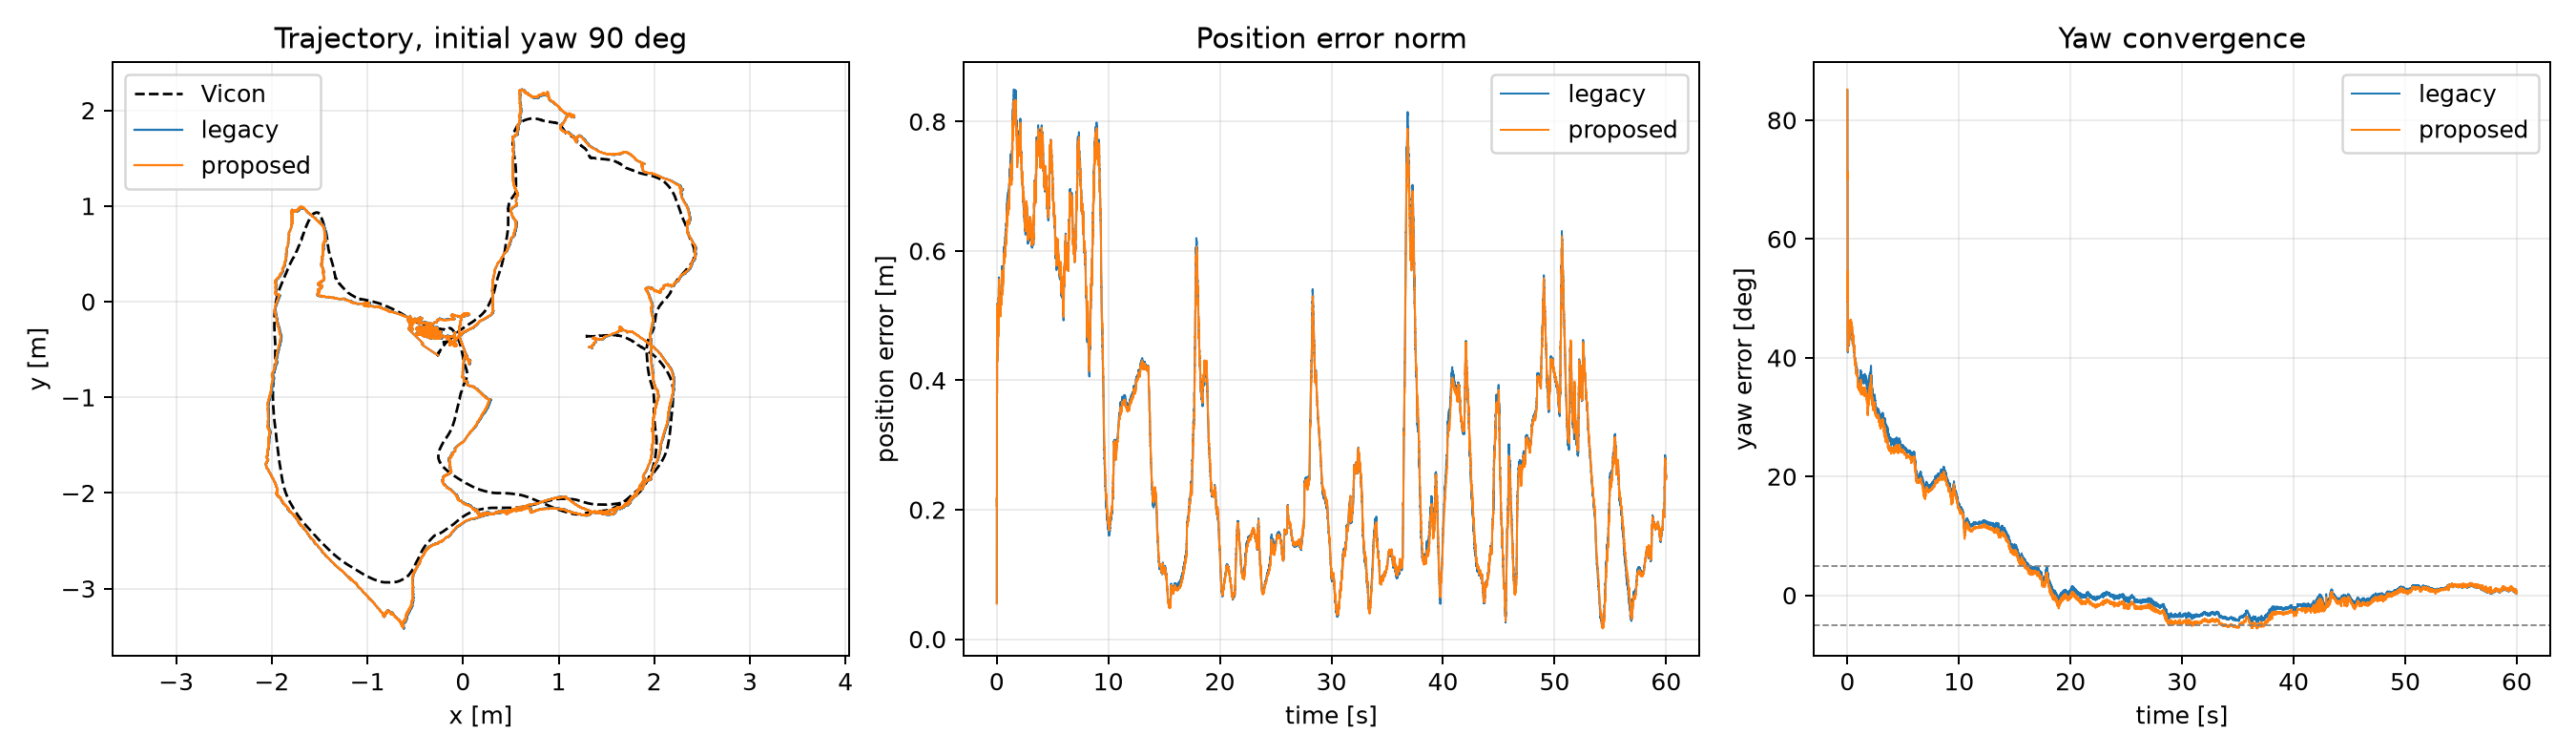
\includegraphics[width=0.98\textwidth]{../imu-uwb-inekf/results/task01_final_fast_const4_60s/comparison_yaw_090.png}
\caption{const4：$90^\circ$ yaw 连续收敛，主要误差峰值与 Legacy 出现在相同运动段。}
\end{figure}

\section{验证与边界}

自动测试 9/9 通过，新增测试确认零角速度更新降低陀螺偏置误差且不改动速度。两张结果图
已目视检查，无发散、非物理跳变或曲线裁切。当前数据无可靠偏置真值，因此不报告偏置
RMSE 或完整 NEES；在线时空标定、连续时间样条和完整右不变 TDoA Jacobian 仍属于后续
研究，不计入本轮成果。

\begin{thebibliography}{9}
\bibitem{li2023continuous} K. Li, Z. Cao, and U. D. Hanebeck,
``Continuous-Time Ultra-Wideband-Inertial Fusion,'' IEEE Robotics and Automation Letters,
vol. 8, no. 7, pp. 4338--4345, 2023, DOI: \href{https://doi.org/10.1109/LRA.2023.3281932}{10.1109/LRA.2023.3281932}.
\bibitem{goudar2021calibration} A. Goudar and A. P. Schoellig,
``Online Spatio-temporal Calibration of Tightly-coupled Ultrawideband-aided Inertial Localization,''
IEEE/RSJ IROS, 2021, \href{https://arxiv.org/abs/2108.00133}{arXiv:2108.00133}.
\bibitem{li2018mav} J. Li et al., ``Accurate 3D Localization for MAV Swarms by UWB and IMU Fusion,''
IEEE ICCA, 2018, DOI: \href{https://doi.org/10.1109/ICCA.2018.8444329}{10.1109/ICCA.2018.8444329}.
\bibitem{kilic2023zu} C. Kilic, E. Gutierrez, and J. N. Gross,
``Evaluation of the Benefits of Zero Velocity Update in Decentralized EKF-Based Cooperative Localization
Algorithms for GNSS-Denied Multi-Robot Systems,'' 2023,
\href{https://arxiv.org/abs/2306.17703}{arXiv:2306.17703}.
\end{thebibliography}

\end{document}
